\section{Concept Mapping}
\label{section:concept}

The core of \emph{GESTALT}'s geospatial search capability resides in what we call the \emph{Concept Mapping} component.
Concept mapping is the process of extracting and explicitly encoding the implicit geographic relationships between objects and locations. 
By encoding these spatial relationships in a manner that can be compared with visual queries issued by the user, we enable a form of spatial last-mile search that (to our knowledge) does not presently exist in any GIS tools.
We implement two forms of concept mapping: object-location concept mapping and object-object concept mapping.
In both cases, concept mapping involves two phases: the encoding phase (offline) and the search phase (online). 
We discuss the details of the encoding phase in this section and leave the search details to section \ref{section:search}.


\subsection{Object-Location relations}
Object-location relations encode whether an object is North, South, East or West of a location. 
This type of information supports simple queries, such as when a user knows that a location has a lake on its western side. 
Each individual object-location relationship is defined independently of other objects associated with that location, and multiple constraints can be combined to form a more specific query, such as a lake west of the location and a pond south of the location.

Figure \ref{figure:ConceptMap-LO} shows how we encode a location (\ref{fig:CM-LO-Example}) as a geospatial index based on realtive position to the location centroid (\ref{fig:CM-LO-Setup}) , and then how queries are processed (\ref{fig:CM-LO-Query}).

To encode a location, we begin by setting the centroid of the location provided by OSM during Data Acquisition to be the root of a quartering of the search space into NorthWest, NorthEast, SouthWest and SouthEast quadrants. 
Each object's coordinates are compared to the location centroid and it is assigned to the appropriate quadrant. 
Where a point lies on the border we adopt the convention that it belongs to the southern and western quadrants. 
To query the location-object index, a user imagines themselves standing at the centre of the location and enters the query terms into the quadrant they believe it belongs in. 
That query map is then compared to each candidate location. An object in the query is in the same quadrant as an object in a candidate location, the number of correct terms increments.
The query returns the count of correct assignments, which are then used to rank the candidate locations from most to fewest matches. 

\begin{figure*}[h]
    \centering
    \begin{subfigure}[t]{.3\textwidth}
        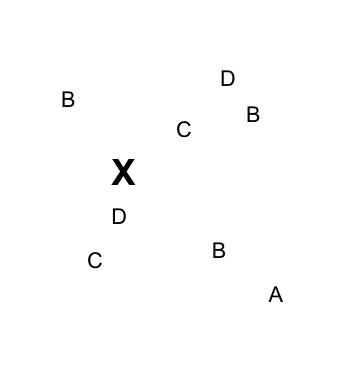
\includegraphics[width=\textwidth]{CM-ExampleLocation.png}
        \caption{\small A candidate location X has named objects A-D with the spatial layout depicted above.} 
        \label{fig:CM-LO-Example}
    \end{subfigure}
    \hfill
    \begin{subfigure}[t]{.3\textwidth}
        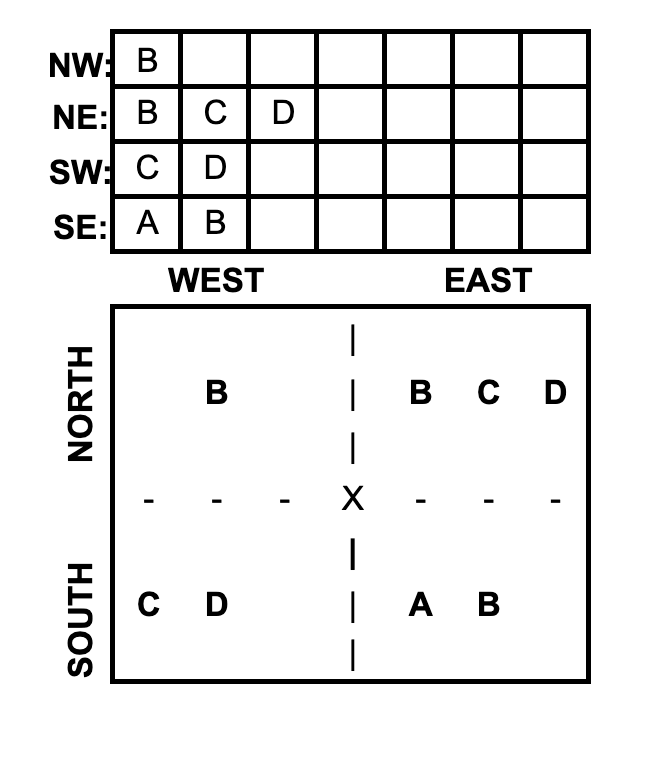
\includegraphics[width=\textwidth]{CM-LO-Setup.png}
        \caption{\small The objects are binned into spatial quadrants based on their relative position to the location centroid, X.} 
        \label{fig:CM-LO-Setup}
    \end{subfigure}
    \hfill
        \begin{subfigure}[t]{.3\textwidth}
        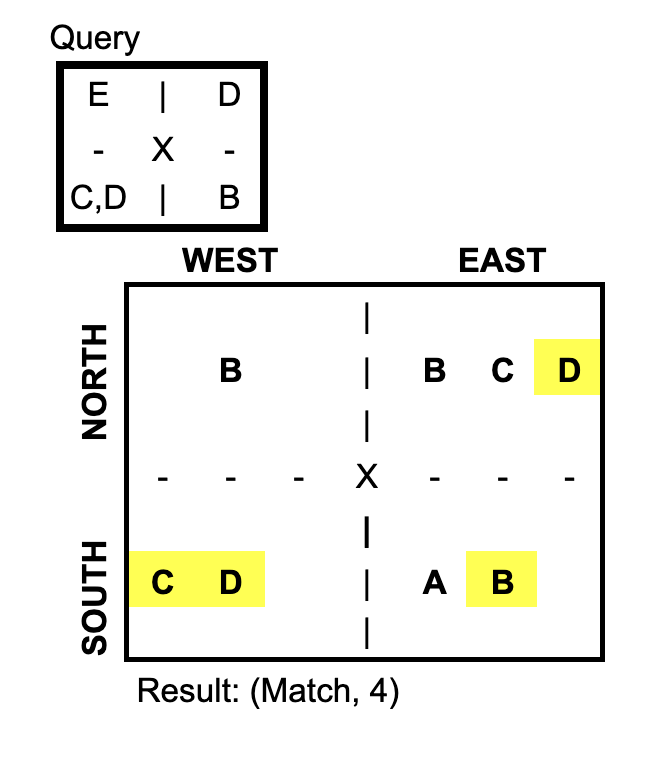
\includegraphics[width=\textwidth]{CM-LO-Query1.png}
        \caption{\small Searching counts the number of query terms that correspond to a location's quadrants and returns the count, allowing multiple candidate solutions to be ranked by closeness of match.}
        \label{fig:CM-LO-Query}
    \hfill
    \end{subfigure}
    \caption{\textbf{Generate and Query an Object-Location Concept Map.}}\label{figure:ConceptMap-LO} 
\end{figure*}



\subsection{Object-object relations}

The other type of spatial relationships \emph{GESTALT} supports searching are object-object relations, which in the genral case are more complex than object-location relations.
Object-object relations refer to a configuration of objects that each relate to one another spatially.
For example, a tree, a pond, and a sign might form a triangle, with each object having a directional constraint with respect to every other object in the query (i.e. tree northwest of pond, pond southeast of sign, and sign southwest of tree).
As the number of objects in the object-object configuration increases, the number of pairwise directional relationships needed to specify the query grows \nrscomment{exponentially??} \osullikomment{I don't think so. Thinking of fully connected graphs, for V:E, 1:0, 2:1, 3:3, 4:6, 5:10, 6:15 ... that's not exponential growth right?}.
As such, object-object relations lend themselves particularly well to pictorial query specification \nrscomment{CITE}.
This method of specifying the spatial positioning of objects aligns nicely with how humans tend to think about and describe landmarks in the world- by drawing a map. 

Figure \ref{figure:ConceptMap-OO} shows how we encode a location (\ref{fig:CM-OO-Example}) as a matrix of relative object positions (\ref{fig:CM-OO-Setup}) , and then how queries are processed (\ref{fig:CM-OO-Query}).

For intuition on this approach, consider the limitations of the location-object approach. 
It assumes that the user knows where the location centroid is and which way north was at that location. 
For large locaitons it doesn't account for a situation were a user may information about objects in one qudrant, limiting their ability to make good matches.  
In these circumstances, we can instead search for the relative position of objects to each other, and ignore their absolute position within the location.
To generate the object-object matrix concept map, we sort all objects from north to south in one list, and all objects west to east in another. Their position in the matrix is then determined by their position in the matrix. For example in figure ref{{fig:CM-OO-Setup}} object \textbf{"A"} is in the 8th position from the North, and the 8th Position from the west, so in the matrix it is assigned to index [0,0].
To then query this sparse matrix, approached it as you might approach looking for something on a map - by eliminating confusing or redundant information until we are left with a very simple question to answer. 
We would probably just zoom in a little closer on our mapping software to see if we can see the arrangement of objects we are looking for - and so our approach mimics the 'zooming-in' approach.
Our implemenation aggressively prunes the search space using recursive grid search \osullikomment{Cite}. In Figure \ref{CM-OO-Query} the query has a "C" object as the most northern object. 
So, we can prune the entire search space north of the north most C, because no matches in that region can satisfy the query. 
Next, recurse and we prune on the matrix from the west, knowing that no terms west of the west-most D can possibly satisfy the query. 
The pruning continues from the north, then the south until there is only a single search term left. 
If that term exists anywhere in the unpruned area, the query matches. 
Note that this approach returns any collection of objects that match the pattern specified in the query, regardless of other objects being present or how many times the sub-pattern occurs in the query space. 

\begin{figure*}[h]
    \centering
    \begin{subfigure}[t]{.3\textwidth}
        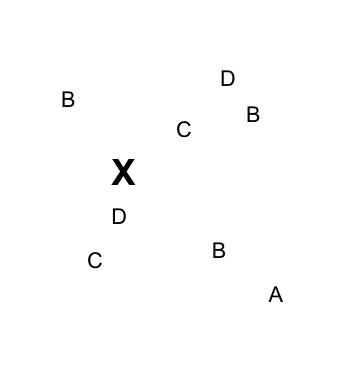
\includegraphics[width=\textwidth]{CM-ExampleLocation.png}
        \caption{\small A candidate location X has named objects A-D with the spatial layout depicted above.}
        \label{fig:CM-Example}
    \end{subfigure}
    \hfill
    \begin{subfigure}[t]{.3\textwidth}
        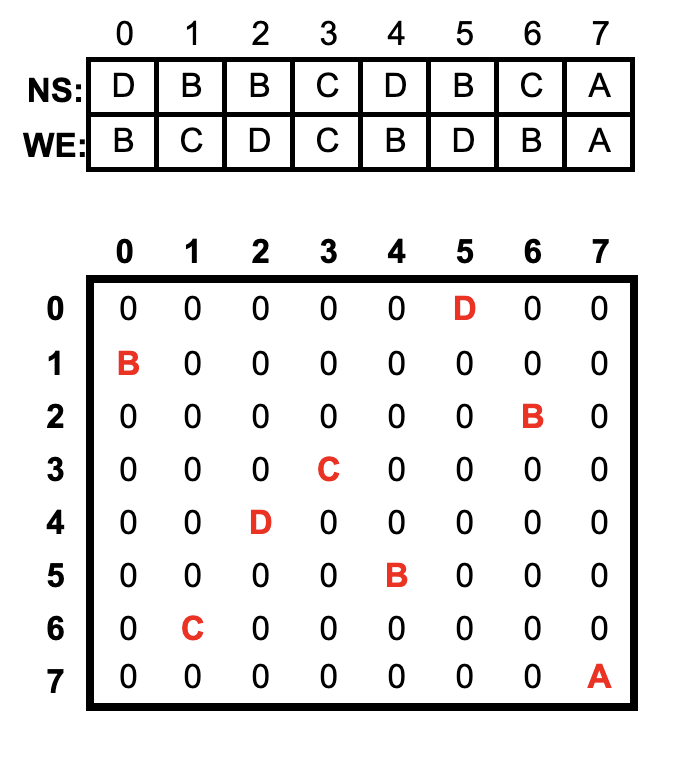
\includegraphics[width=\textwidth]{CM-OO-Setup.png}
        \caption{\small During pre-processing, the objects associated with location X are ordered North to South (NS) and West to East (WE) and mapped into a matrix with corresponding indices.}
        \label{fig:CM-OO-Setup}
    \end{subfigure}
    \hfill
        \begin{subfigure}[t]{.3\textwidth}
        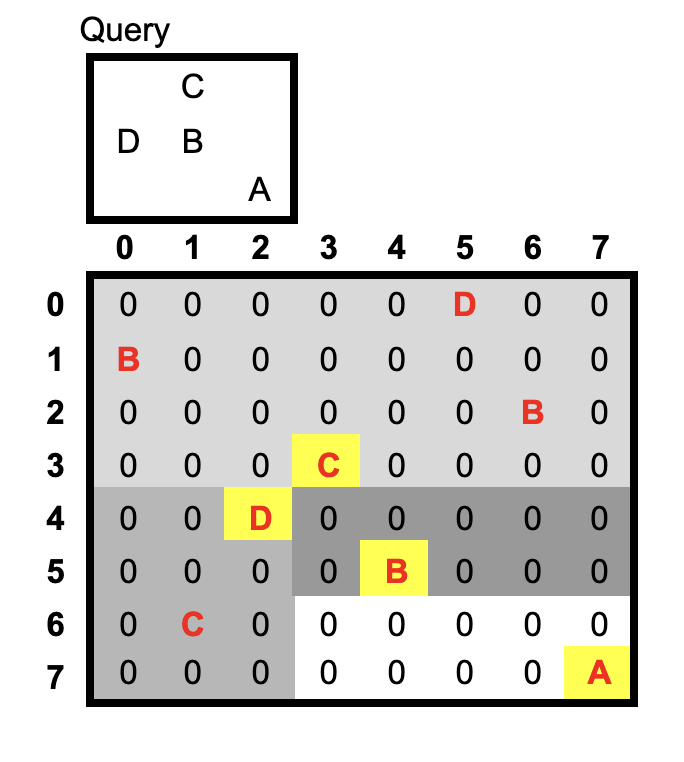
\includegraphics[width=\textwidth]{CM-OO-Query1.png}
        \caption{\small Searching recursively prunes for ANY match. Each recursion is a darker shade, with unpruned area in white. Objects highlighted in yellow are found to match the query configuration; candidate location X is a match for the query.}
        \label{fig:CM-OO-Query}
    \hfill
    \end{subfigure}
    \caption{\textbf{Generate and Query an Object-Object Concept Map.}}\label{figure:ConceptMap} 
\end{figure*}

\begin{figure*}[h]
    \centering
    \begin{subfigure}[t]{.2\textwidth} 
        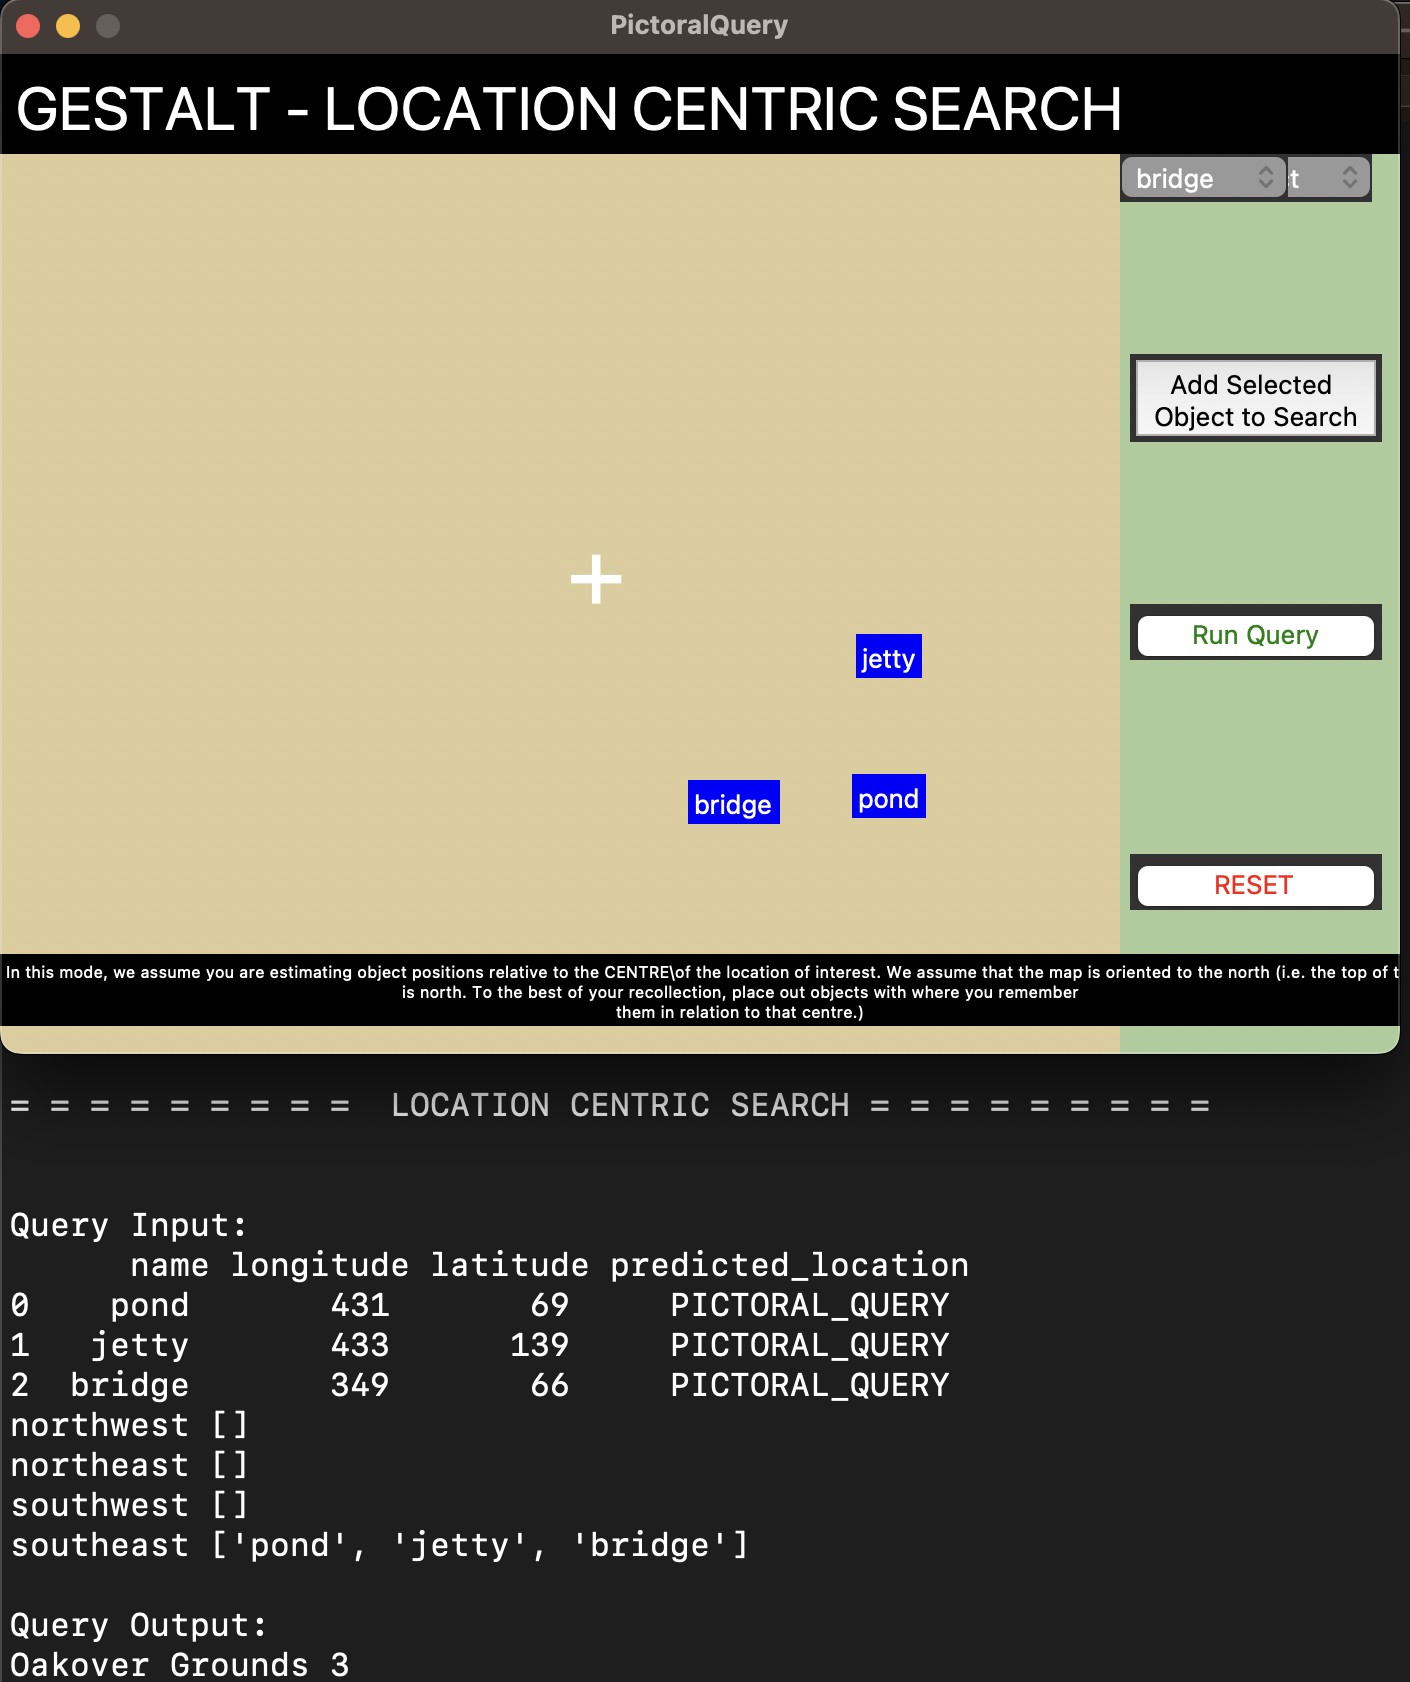
\includegraphics[width=\textwidth]{GUI-LO.png}
        \caption{\small The Location Object GUI uses the nominal centre of the location "+" to divide the search space into quadrants.}
        \label{fig:GUI-LO}
    \end{subfigure}
    \hfill
    \begin{subfigure}[t]{.2\textwidth} 
        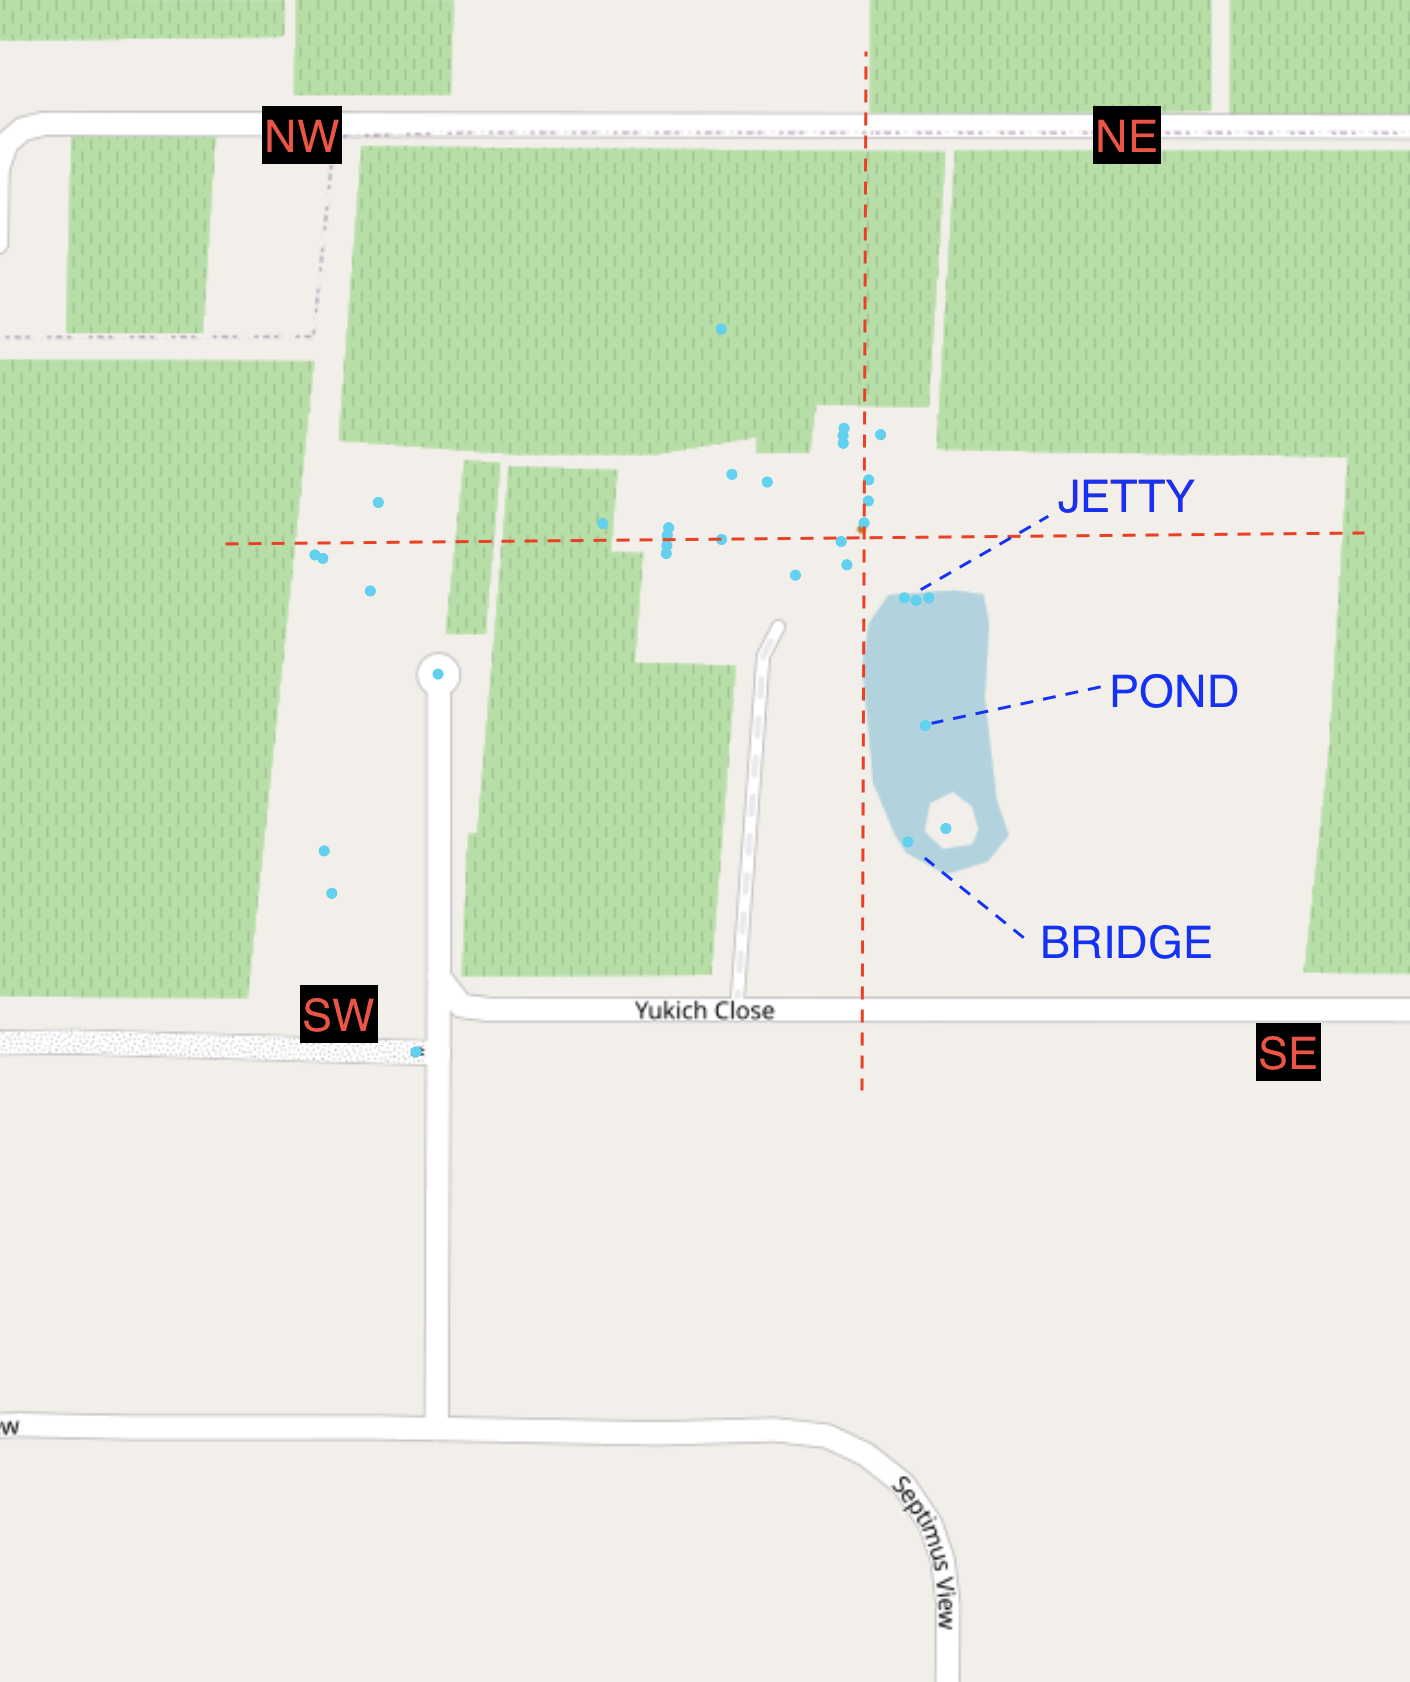
\includegraphics[width=\textwidth]{LO-Ground-Truth.png}
        \caption{\small The location of the Oakover coordinates shows that it won't necessarily be the centre of the object cluster that the space is subdivided on.}
        \label{fig:LO-Ground-Truth}
    \end{subfigure}
    \hfill
    \begin{subfigure}[t]{.2\textwidth}
        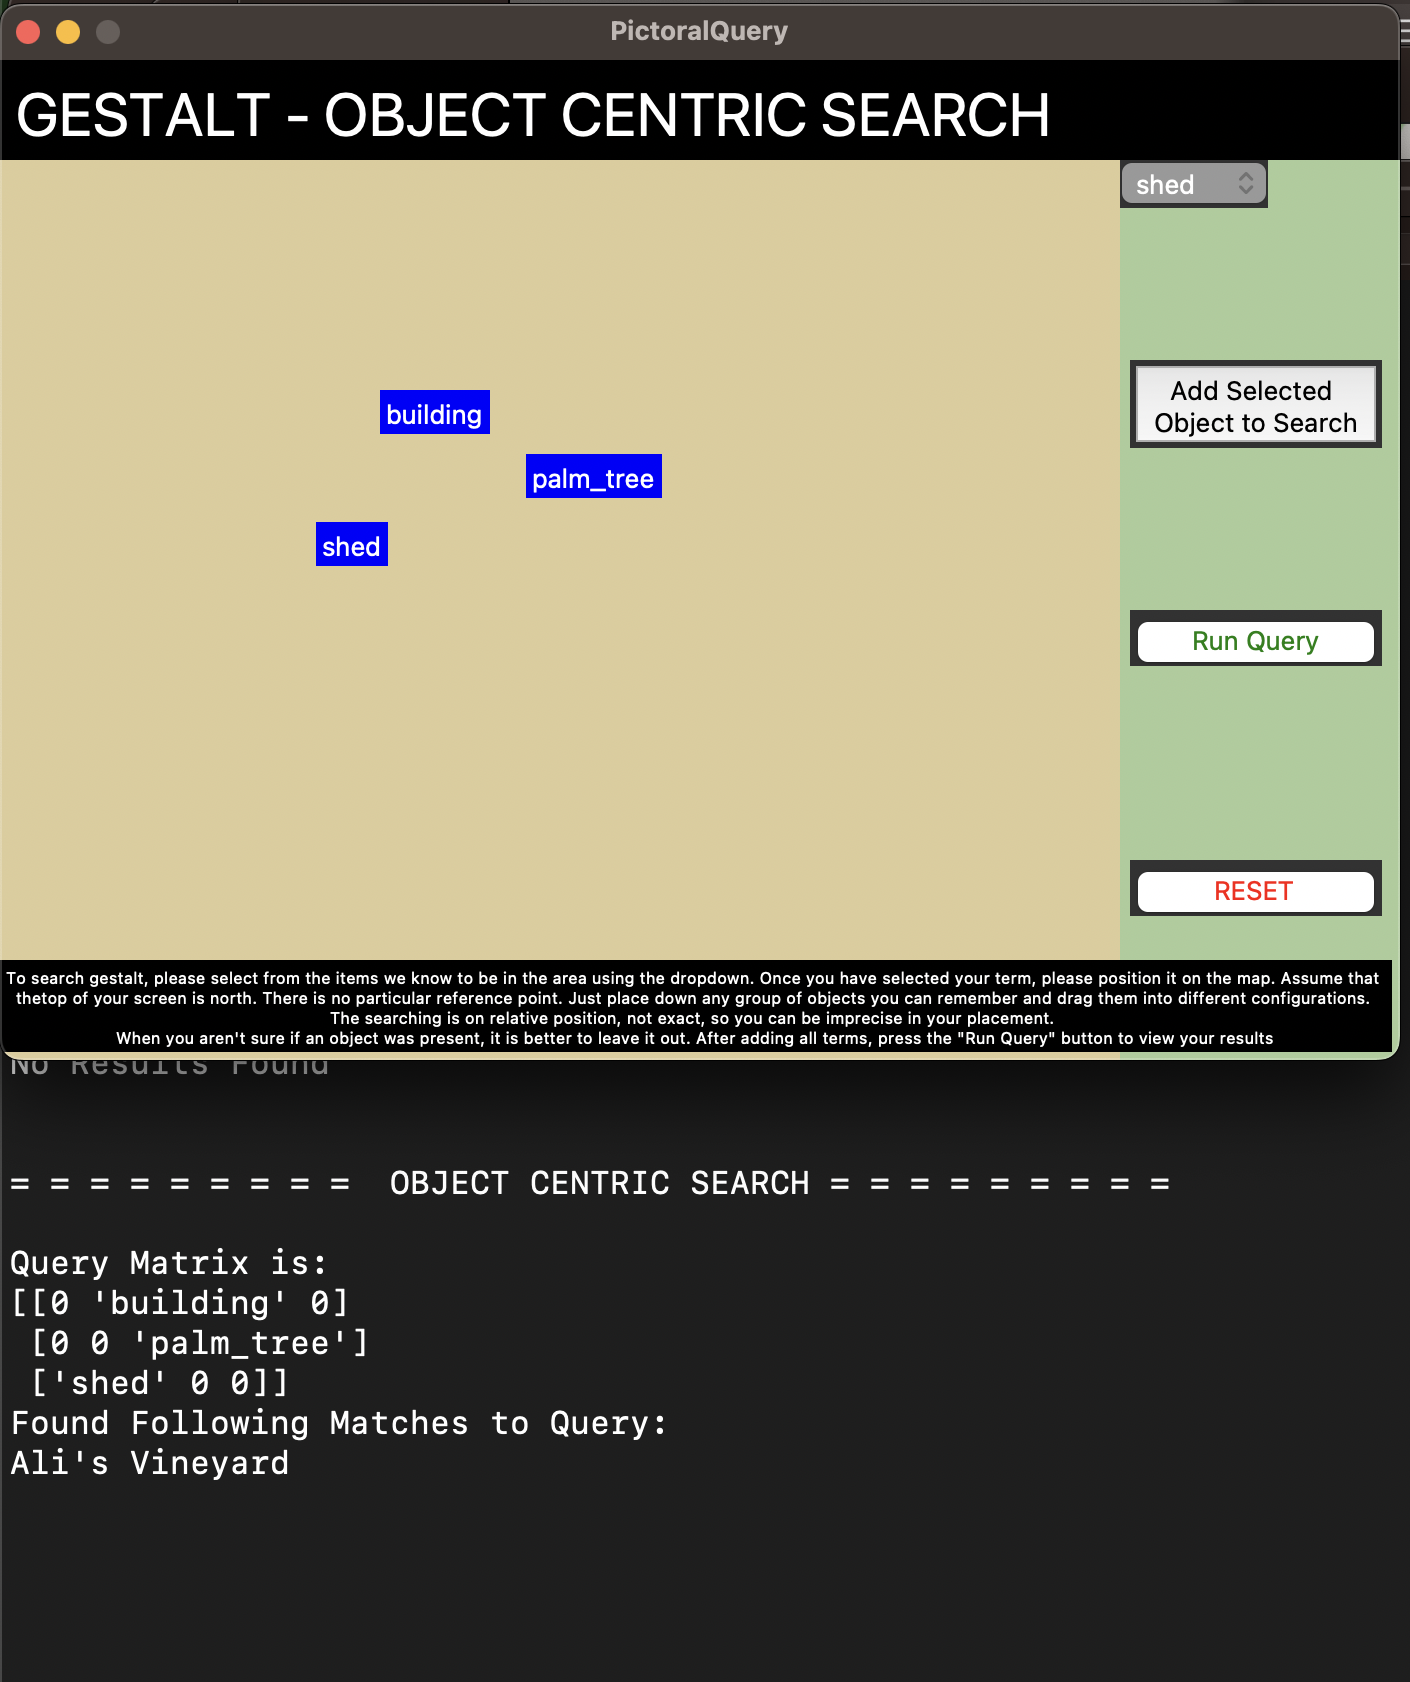
\includegraphics[width=\textwidth]{GUI-OO.png}
        \caption{\small The Object Object GUI allows users to arrange objects in any manner they see fit.}
        \label{fig:GUI-OO}
    \end{subfigure}
    \begin{subfigure}[t]{.2\textwidth} 
        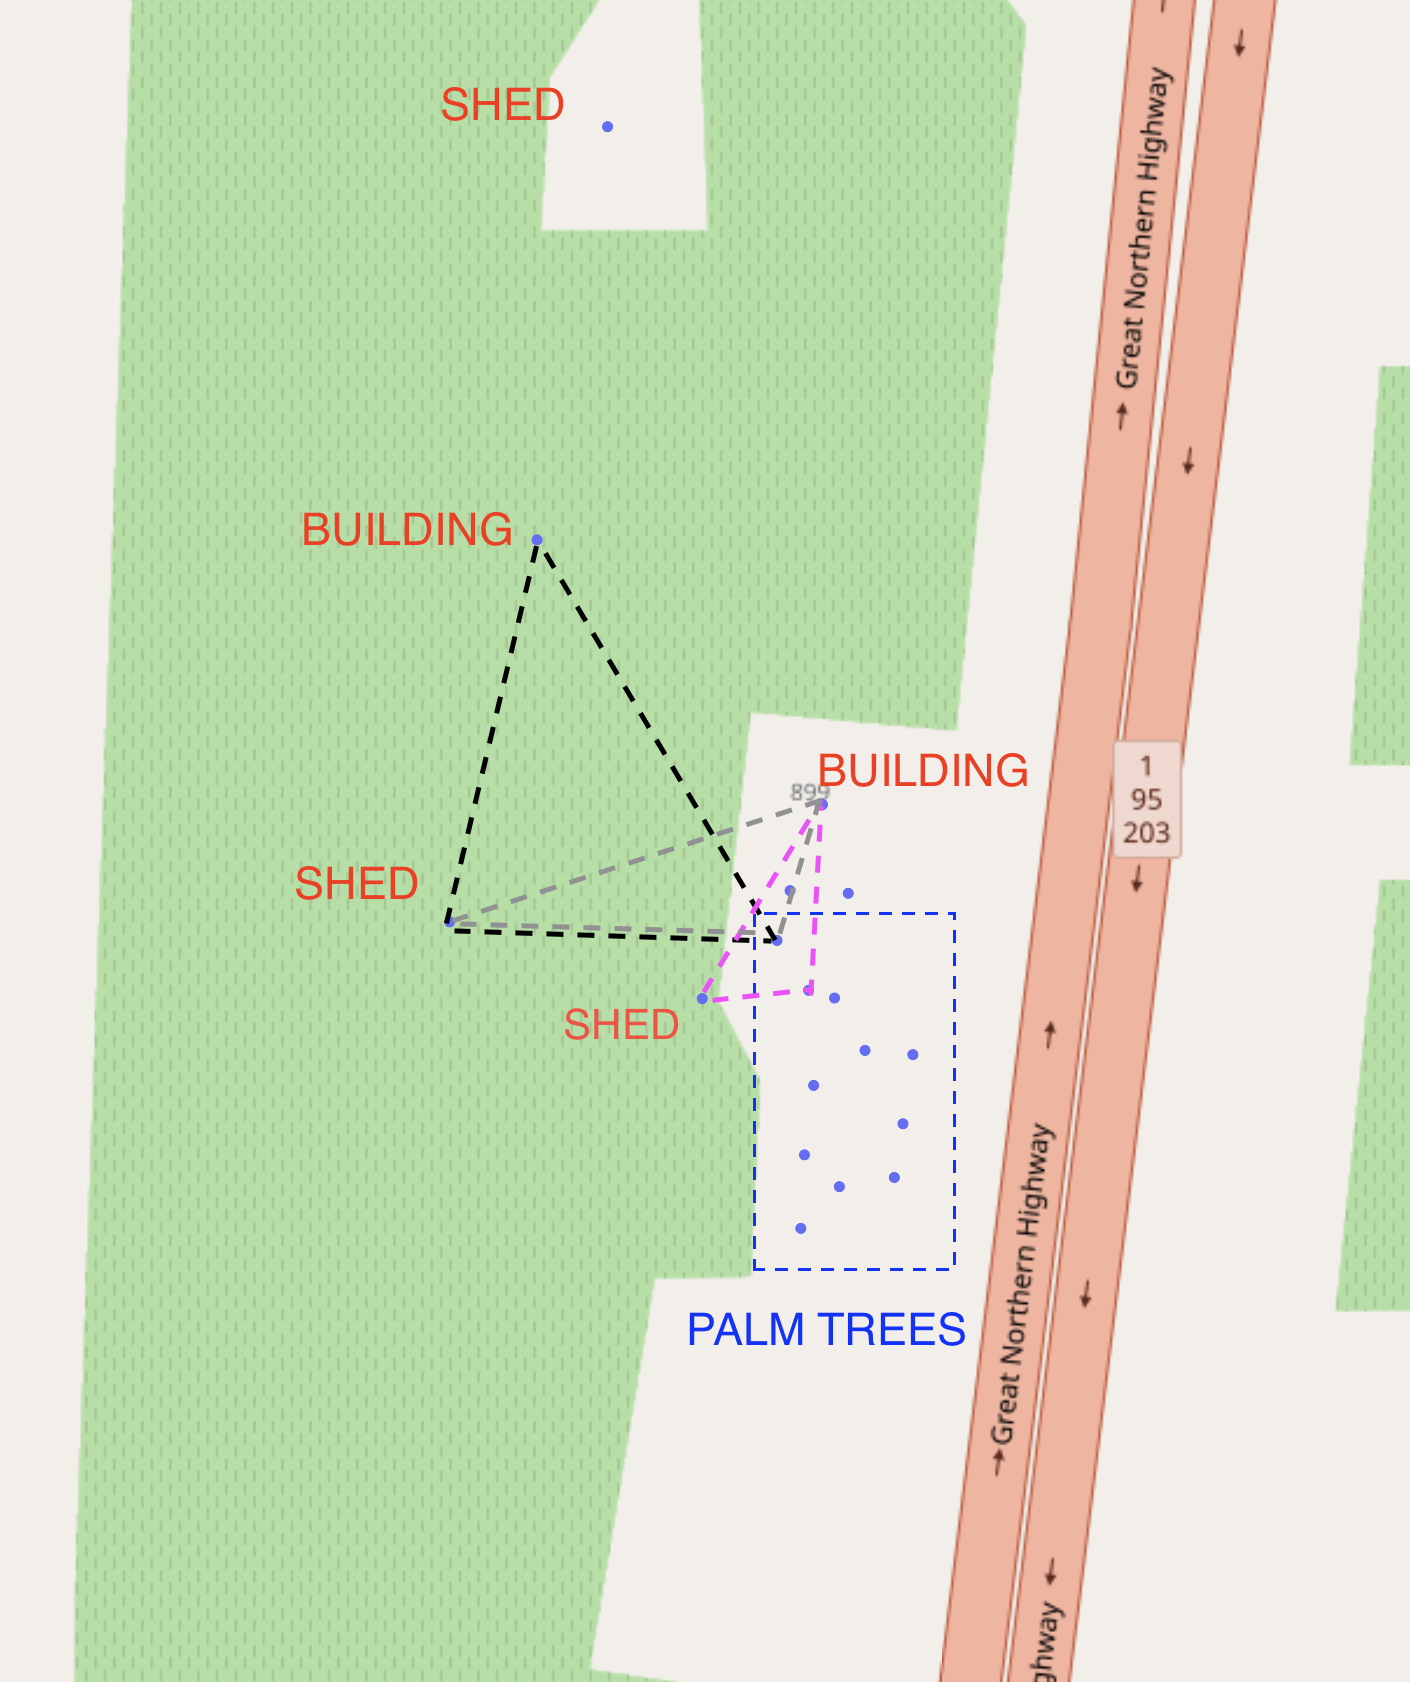
\includegraphics[width=\textwidth]{OO-Ground-Truth.png}
        \caption{\small The triangles show matching candidatesm any of which would cause the query to return true.}
        \label{fig:OO-Ground-Truth}
    \end{subfigure}
    \hfill
    \caption{\textbf{Users of the prototype Pictorial Query interface in both modes add objects from the drop-down menu and position them on the screen by dragging the lables. Beneath each window is the encoded query and the result from searching GESTALTs database. The Pictoral Query Interface allows users of GESTALT to mimic how they would explain features of location to another person, in this case by drawing a quick map.}}\label{figure:GUI} 
\end{figure*}

\subsection{Encoding the Spatial Relationships of objects and locations}

\subsubsection{Object-location encoding}
Object-Location concept maps are encoded as a per-location index that subdivides the search space into four quadrants - NorthWest, NorthEast, SouthWest and SouthEast, splitting on the centroid of the location. The divison of space aims to emulate how people tend to relate the world to their position in it geospatially, 


\subsubsection{Object-object encoding}
Rather than use a fully-connected graph, we encode both the locations, and later, the pictorial query inputs as matrices with zeros representing unallocated space and the names of objects. 
The matrices are $NxN$, where $N$ is the number of objects at a location. 
Using algorithm \ref{alg:geoToGrid}, we assign each object in a given location to a position $(i,j)$ in the Matrix where $i$ is its order of appearance from north to south and $j$ is the same object's order of appearance from west to east. 
The result is a matrix in which each row and column has only a single object. 
Where ties are experienced in the real world (due to a lack of GPS precision, or very close position) they are broken lexicographically in the object-object concept map instantiation.
%The process of creating and querying a concept map is shown in Figure \ref{figure:ConceptMap}.



% This all belongs in search
%\subsubsection{Query Input}
%- algorithm for parsing from grid, etc.
%\subsubsection{Solution}
%- recursive algorithm for finding any match
%- complexity analysis
%
%\subsubsection{Experimental Results?}
%- on ground truth queries? report number of locations pruned? timings?

%Concept mapping has been partially implemented in Python leveraging the \textit{Scipy} library\footnote{\href{https://pypi.org/project/scipy/}{SciPy PyPI Repo}}. Two different approaches have been trialed. 
%The first is simple dynamic arithmetic on the coordinates stored in a Pandas data frame. If one set of coordinates is above, below, left or right of another, it is north, south, east or west, respectively. 
%While these calculations are in constant time for straightforward comparisons of known objects (e.g. "is the pond west of the bridge"), the time complexity rapidly increases as soon as aggregations are employed. 
%Queries of "Give me everything west of the duck pond" would execute in $O(N)$ time as each element has to be examined. Worst-case queries would run in $O(N\sup{2})$ time, where every object is checked for its position relative to every other object. 

%The second (better) approach (only partially implemented) instantiates the objects within a location into a KD-Tree. 
%Assuming that the object centroid is the root, we can quickly complete queries like "Give me everything west of the duck pond" by leveraging the structure of the subtrees to return the requested set. 
%Similarly, getting the relative positions of two objects searches for a common ancestor. It uses the path between the children and their ancestor node to infer their spatial relation to each other.

%A third approach, designed to leverage the \textit{Neo4J Python Library}\footnote{\href{https://pypi.org/project/neo4j/}{Neo4J PyPI Repo}} to connect to a \textit{Neo4J Graph Database}\footnote{\href{https://neo4j.com/}{Neo4J Website}} but not implemented frames concept mapping as a graph traversal problem. 
%In this formulation, each object is a node on a graph. Weighted, labeled edges exist between each node within a given proximity threshold to the node. 
%The edge labels describe the neighboring node's cardinal direction and the distance weights. 
%After constructing the object graph, queries for 'give me everything west of the duck pond' would freely explore nodes connected by west, north and south edges. 
%It can only traverse along an east edge so long as the total cost of traveling east would be less than the cumulative value of the 'west' travel up to this point. 

%%Overall, concept mapping aims to enable geographic search over objects by explicitly representing their geospatial relationships to each other. 
%The author implemented a very basic approach using coordinate arithmetic was quickly determined to be infeasible for the extensive data sets that \textit{GESTALT} anticipates processing. 
%KD-Trees for the objects in each location have been implemented, as have the KD-Trees for the locations themselves. 
%This conceptual KD-Tree of KD-Trees approach performs a natural aggregation function which, provided that regions are created consistently, will allow for relative spatial queries at different levels of granularity. 
%Empirical evaluation of the performance of the arithmetic, KD-Tree and Graph-based approaches is yet to be completed. 


%%%%%%%%%%%%%%%NSCH clean up, incorporate, and delete the text below this point
%The first is \textit{Static Cardinal Relations} which encodes whether an object is North, South, East or West of a location. Static Cardinal Relations support simple queries where the user knows that a location has a lake on its western side. 
%The second is \textit{Dynamic Cardinal Relations} which determines whether an object is North, South, East or West of another object within a location. These queries support cases where a searcher might remember standing at a lake northeast of a location and that there was a swingset to the immediate west of them but still in the northeast of the location overall. 


%Concept mapping needs to be unsupervised and support aggregation. Tracking every object's relative location to every other object quickly becomes intractable, so mechanisms to aggregate depending on the level of granularity need to be applied. 
%Accordingly, the underlying data structure must support aggregation and relative position querying. 